\documentclass{beamer}
\usepackage[utf8]{inputenc}

\usetheme{Madrid}
\usecolortheme{default}
\usepackage{amsmath,amssymb,amsfonts,amsthm}
\usepackage{txfonts}
\usepackage{tkz-euclide}
\usepackage{listings}
\usepackage{adjustbox}
\usepackage{array}
\usepackage{tabularx}
\usepackage{gvv}
\usepackage{lmodern}
\usepackage{circuitikz}
\usepackage{tikz}
\usepackage{graphicx}
\usepackage{mathtools}

\setbeamertemplate{page number in head/foot}[totalframenumber]

\usepackage{tcolorbox}
\tcbuselibrary{minted,breakable,xparse,skins}



\definecolor{bg}{gray}{0.95}
\DeclareTCBListing{mintedbox}{O{}m!O{}}{%
  breakable=true,
  listing engine=minted,
  listing only,
  minted language=#2,
  minted style=default,
  minted options={%
    linenos,
    gobble=0,
    breaklines=true,
    breakafter=,,
    fontsize=\small,
    numbersep=8pt,
    #1},
  boxsep=0pt,
  left skip=0pt,
  right skip=0pt,
  left=25pt,
  right=0pt,
  top=3pt,
  bottom=3pt,
  arc=5pt,
  leftrule=0pt,
  rightrule=0pt,
  bottomrule=2pt,
  toprule=2pt,
  colback=bg,
  colframe=orange!70,
  enhanced,
  overlay={%
    \begin{tcbclipinterior}
    \fill[orange!20!white] (frame.south west) rectangle ([xshift=20pt]frame.north west);
    \end{tcbclipinterior}},
  #3,
}
\lstset{
    language=C,
    basicstyle=\ttfamily\small,
    keywordstyle=\color{blue},
    stringstyle=\color{orange},
    commentstyle=\color{green!60!black},
    numbers=left,
    numberstyle=\tiny\color{gray},
    breaklines=true,
    showstringspaces=false,
}
\title{5.8.43}
\date{28th September, 2025}
\author{Puni Aditya - EE25BTECH11046}

\begin{document}

\frame{\titlepage}
\begin{frame}{Question}
The sum of three numbers is 6. If we multiply the third number by 3 and add the second number to it, we get 11. By adding the first and third numbers, we get double of the second number. Find the numbers.
\end{frame}

\begin{frame}{Theoretical Solution}
Given
\begin{align}
    x+y+z &= 6 \\
    0x+y+3z &= 11 \\
    x-2y+z &= 0
\end{align}
\begin{align}
    \myaugvec{3}{
        1 & 1 & 1 & 6 \\
        0 & 1 & 3 & 11 \\
        1 & -2 & 1 & 0
    }
    \xleftrightarrow{\text{R}_3 \to \text{R}_3 - \text{R}_1}
    \myaugvec{3}{
        1 & 1 & 1 & 6 \\
        0 & 1 & 3 & 11 \\
        0 & -3 & 0 & -6
    }
\end{align}
\begin{align}
    \xleftrightarrow{\text{R}_3 \to -\frac{1}{3}\text{R}_3}
    \myaugvec{3}{
        1 & 1 & 1 & 6 \\
        0 & 1 & 3 & 11 \\
        0 & 1 & 0 & 2
    }
    \xleftrightarrow{\text{R}_2 \leftrightarrow \text{R}_3}
    \myaugvec{3}{
        1 & 1 & 1 & 6 \\
        0 & 1 & 0 & 2 \\
        0 & 1 & 3 & 11
    }
\end{align}
\end{frame}

\begin{frame}{Theoretical Solution}
\begin{align}
    \xleftrightarrow[\text{R}_3 \to \text{R}_3 - \text{R}_2]{\text{R}_1 \to \text{R}_1 - \text{R}_2}
    \myaugvec{3}{
        1 & 0 & 1 & 4 \\
        0 & 1 & 0 & 2 \\
        0 & 0 & 3 & 9
    }
    \xleftrightarrow{\text{R}_3 \to \frac{1}{3}\text{R}_3}
    \myaugvec{3}{
        1 & 0 & 1 & 4 \\
        0 & 1 & 0 & 2 \\
        0 & 0 & 1 & 3
    }
\end{align}
\begin{align}
    \xleftrightarrow{\text{R}_1 \to \text{R}_1 - \text{R}_3}
    \myaugvec{3}{
        1 & 0 & 0 & 1 \\
        0 & 1 & 0 & 2 \\
        0 & 0 & 1 & 3
    }
\end{align}
\end{frame}

\begin{frame}{Example}
\begin{align*}
    \myvec{x \\ y \\ z} = \myvec{1 \\ 2 \\ 3}
\end{align*}
$\therefore$ The required numbers are 1,2 and 3.
\end{frame}

\begin{frame}{Plot}
    \begin{figure}
        \centering
        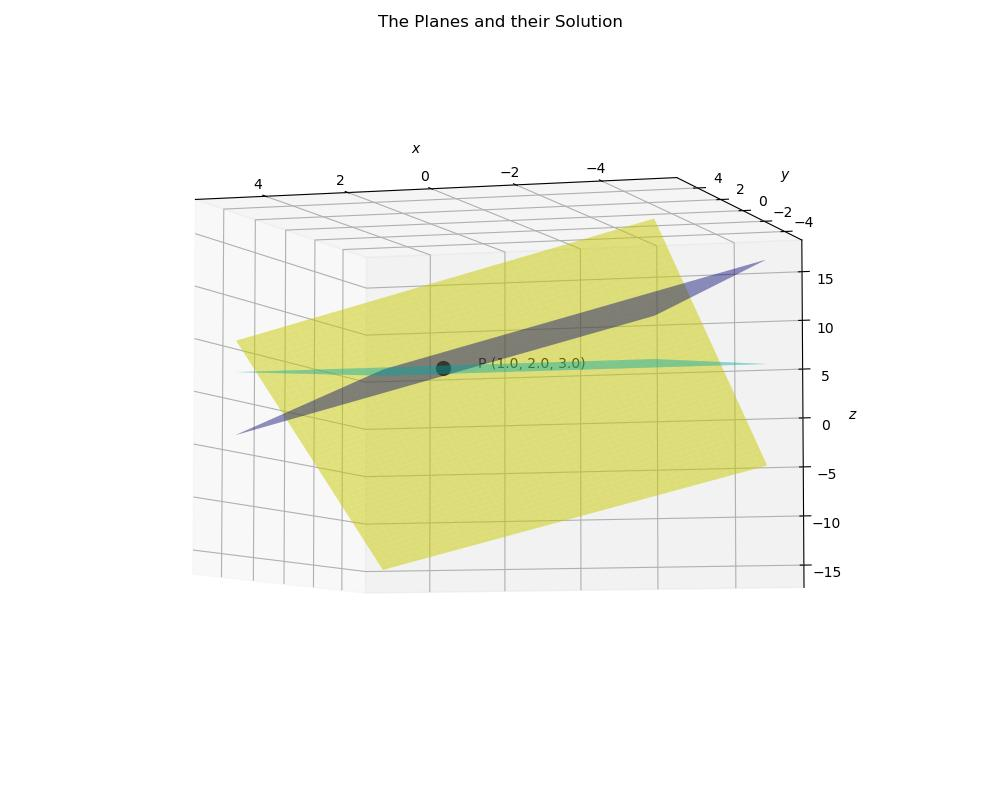
\includegraphics[width=0.5\columnwidth]{../figs/plot_c.jpg}
        \caption{Plot}
        \label{fig:fig}
    \end{figure}
\end{frame}

\end{document}
